\chapter{深度伪造的研究工具与检测手段的分类}
\label{chap:3}

本章节探讨深度伪造的研究工具与检测手段的分类,首先会根据 Thanh Thi Nguyen 等人 \cite{https://doi.org/10.48550/arxiv.1909.11573} 所进行的研究工作的简述,在他们的工作总结中将其工具分为两大类,也就是图像检测与人脸视频检测,并有着详细的整理,此外根据 Li XR 等人近期对深度伪造与检测的汇整工作\cite{2021496} 也有着详尽的说明,本作业除了针对究工具与检测手段等研究者们的近来工作将其汇整于此章。

\begin{figure}[htb]
\centering 
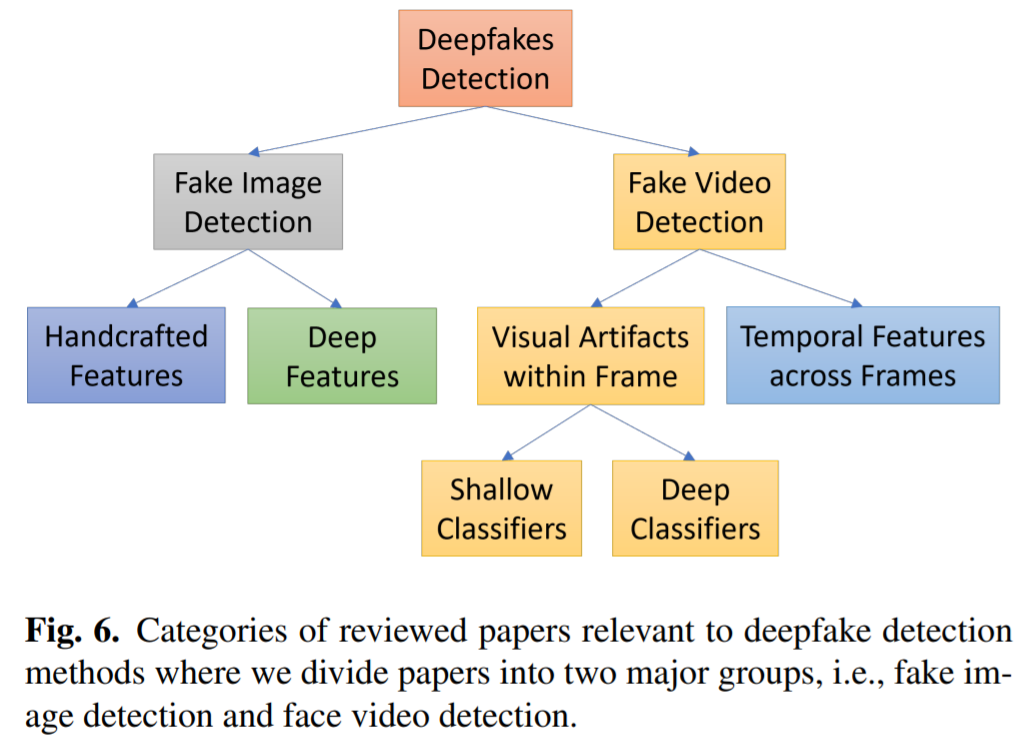
\includegraphics[width=0.90\textwidth]{img/ch3m1.png} 
\caption{从由 Thanh Thi Nguyen 等人 \cite{https://doi.org/10.48550/arxiv.1909.11573} 将深度伪造的伪造分为两大类}
\label{Test}
\end{figure}


\section{深度伪造的图像检测与人脸视频检测整理}

根据由 Thanh Thi Nguyen 等人 \cite{https://doi.org/10.48550/arxiv.1909.11573}的在深度伪造的工作中所整理的分类整理的过程中将其分为了图像检测与人脸视频检测。同时该工作也有将其深度伪造的检测手段进行总结,本作业根据原总结工作再汇整为深度伪造检测手段整理两表,两表之中总共有 24 种检测手段,这当中又因该工作所进行的分类,而分为三部分,其一为针对图像的检测,列于表二,共有 9 种手段,其二为影像的检测手段,其列于表一,共有 13 种手段,其三为图像检测与人脸视频检测皆可的检测,只有两种手段,并与表二图像检测并列。



%\begin{table}[ht]
%  \caption{test}
%  \label{Tab:bookRWCal}
%  \centering
%  \begin{tabular}{lp{3cm}p{3cm}p{3cm}}
%  \toprule
%  \textbf{著作类别} &\textbf{A级出版社} &\textbf{B级出版社}&\textbf{C级出版社}\\
%  \midrule
%  学术专著         &第一作者3分/万字,其他作者 2分/万字	&第一作者3分/万字,其他作者 2分/万字	&第一作者3分/万字,其他作者 2分/万字\\
%  \bottomrule
%  \end{tabular}
%\end{table}

\begin{table}[ht]
  \caption{深度伪造检测手段整理}
  \label{Tab:bookRWCal}
  \centering
  %\begin{tabular}{lp{3cm}p{2cm}p{2cm}}
  \begin{tabular}{p{3cm}p{3cm}p{3cm}p{3cm}}
  \toprule
  \textbf{方法} &\textbf{技術} &\textbf{检测种类}&\textbf{备注}\\
  \midrule
 Eye blinking & LRCN & Videos & Yuezun Li 等人\\
 Intra-frame and temporal inconsistencies & CNN and LSTM & Videos & David Guera 等人\\
 Using face warping artifacts & VGG16, ResNet models & Videos & Yuezun Li 等人\\
 MesoNet & CNN & Videos & Darius Afchar 等人\\
 Eye, teach and facial texture & Logistic regression and neural network(NN) & Videos & Falko Matern 等人\\
 Spatio-temporal features with RCN & RCN & Videos & Ekraam Sabir 等人\\
 Spatio-temporal features with LSTM & Convolutional bidirectional recurrent LSTM network & Videos & Akash Chintha 等人\\
 Analysis of PRNU & PRNU & Videos & Marissa Koopman 等人\\
 Phoneme-viseme mismatches & CNN & Videos & Shruti Agarwal 等人\\
 Using attributionbased confidence (ABC) metric & ResNet50 model, pre-trained on VGGFace2 & Videos & Steven Fernandes 等人\\
 Using appearance and behaviour & Rules based on facial and behavioural features & Videos &  Shruti Agarwal 等人\\
 FakeCatcher & CNN & Videos & Umur Aybars Ciftci 等人\\
 Emotion audiovisual affective cues & Siamese network & Videos & Trisha Mittal 等人\\
  \bottomrule
  \end{tabular}
\end{table}

\begin{table}[ht]
  \caption{深度伪造检测手段整理(续)}
  \label{Tab:bookRWCal}
  \centering
  %\begin{tabular}{lp{3cm}p{2cm}p{2cm}}
  \begin{tabular}{p{3cm}p{3cm}p{3cm}p{3cm}}
  \toprule
  \textbf{方法} &\textbf{技術} &\textbf{检测种类}&\textbf{备注}\\
  \midrule
 Head poses & SVM & Videos and Images & Xin Yang 等人\\
 Capsule-forensics & Capsule networks & Videos and Images & Huy H Nguyen 等人\\
 Preprocessing combined with deep network & DCGAN, WGAN-GP and PGGAN. & Images & Xinsheng Xuan 等人\\
 Analyzing convolutional traces & KNN, SVM, and linear discriminant analysis (LDA) & Images &  Luca Guarnera 等人\\
 Bag of words and shallow classifiers & SVM, RF, MLP & Images & Ying Zhang 等人\\
 Pairwise learning & CNN concatenated to CFFN & Images & Chih-Chung Hsu 等人\\
 Defenses against adversarial perturbations in deepfakes & VGG and ResNet & Images &  Apurva Gandhi 等人\\
 Face X-ray & CNN & Images & Chih-Chung Hsu 等人\\
 Using common artifacts of CNN-generated images & ResNet-50 pre-trained with ImageNet & Images & Sheng-Yu Wang 等人\\
 Using convolutional traces on GAN-based images & KNN, SVM, and LDA & Images & Luca Guarnera 等人\\
 Using deep features extracted by CNN & A new CNN model, namely SCnet & Images & Zhiqing Guo 等人\\
  \bottomrule
  \end{tabular}
\end{table}

\section{过往传统的检测手段}


\section{人类的生理特征的检测手段}


\section{图像伪造后留下痕迹的检测手段}


\section{ GAN 模型所产生的检测手段}


\section{图片的深度学习之检测手段}


\section{影像的深度学习之检测手段}















